\chapter{Introducción}

Los algoritmos evolutivos son métodos de optimización y búsqueda de soluciones basados en la Teoría de la Evolución de las especies. Según ésta, un conjunto de individuos forma una generación y éstos, al reproducirse entre ellos, generan nuevos individuos con características comunes de ambos padres.

Actualmente existe una gran cantidad de aplicaciones que hacen uso de los algoritmos evolutivos para toda clase de tareas; desde estrategias de búsqueda a problemas de optimización.


Un subtipo de los problemas de optimización son los problemas de optimización cuadrática, o \textit{QAP}\footnote{Quadratic Asignation Problem} por sus siglas en inglés,  que son problemas de optimización combinatoria. Dicho problema puede describirse de la siguiente forma.


Supongamos que queremos decidir dónde construir \texttt{n} instalaciones (p.ej. fábricas) y tenemos \texttt{n} posibles localizaciones en las que podemos construir dichas instalaciones. Conocemos las distancias que hay entre cada par de instalaciones y también el flujo de materiales que ha de existir entre ellas. El problema consiste en decidir dónde ubicar cada fábrica para minimizar el coste de transporte de materiales.


Formalmente, si llamamos \texttt{d(i, j)} a la distancia de la localización \texttt{i} a la localización \texttt{j} y \texttt{w(i, j)} al peso asociado al flujo de materiales que ha de transportarse de la instalación \texttt{i} a la instalación \texttt{j}, hemos de encontrar la asignación de instalaciones a localizaciones que minimice la función de coste

\[ \sum_{i,j} w(i,j) d(p(i),p(j)) \]
\label{formula:sum}

donde \texttt{p()} define una permutación sobre el conjunto de instalaciones.

El ejemplo clásico de este tipo de problemas es el \textit{TSP}\footnote{Travel Salesman Problem} o Problema del Viajante, donde el objetivo es encontrar la ruta más corta entre varias ciudades.


\begin{figure}[H]
  \centering
  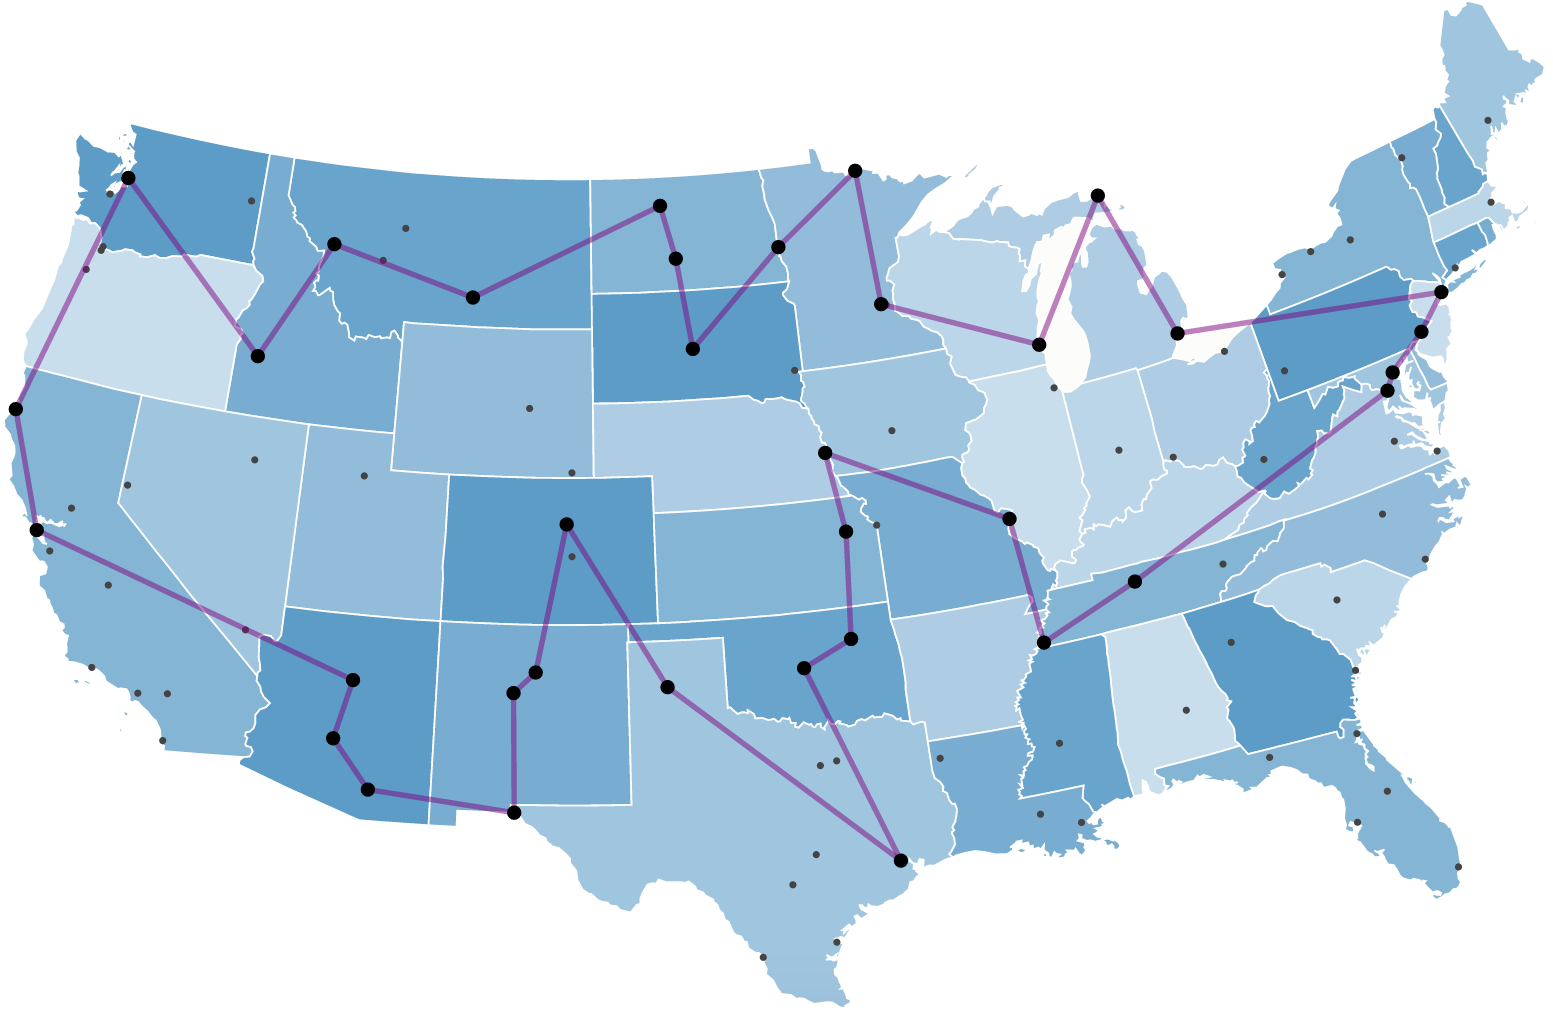
\includegraphics[width=0.65\textwidth]{../images/tsp}
  \caption{Ejemplo de rutas entre ciudades}
  \label{fig:tsp}
\end{figure}


Los casos de prueba para comprobar el funcionamiento de las distintas heurísticas se han obtenido de la biblioteca \textit{QAPLIB}\footnote{\url{(http://www.seas.upenn.edu/qaplib/}}. Cada uno de los archivos contiene el tamaño del problema, la matriz de flujo y la matriz de distancias.

En esta práctica sólo se trabajará con el archivo \texttt{tai256c}, cuyo tamaño es de 256. A día de hoy, la cota inferior global conocida (la mejor solución que se ha obtenido) tiene un fitness de 44,095,032, por lo que se supondrá que cualquier resultado que se obtenga menor a este será erróneo.


\section{Entorno de desarrollo}

Mi ordenador personal, en el cual se ha realizado esta práctica, cuenta con las siguientes características.

\begin{itemize}
  \item \textbf{Sistema operativo}. Windows 10 Educational
  \item \textbf{Procesador}. Intel Core i7-6700HQ Quad-Core 2.6GHz
  \item \textbf{Cache}. 6M
  \item \textbf{Memoria RAM}. 8GB DDR4 2,133MHz
  \item \textbf{Tarjeta gráfica}. NVIDIA 950M 
  \item \textbf{Disco duro}. SanDisk SSD Plus 256GB
  \item \textbf{Lenguaje de programación}. Python 3.7
\end{itemize}

\section{Repositorio}

El desarrollo y la evolución de esta práctica pueden verse en el siguiente repositorio.

\begin{center}
\url{https://github.com/gomezportillo/qap}
\end{center}